\documentclass{beamer}
\usetheme{Boadilla}
% \usepackage{beamerthemesplit} // Activate for custom appearance
\usepackage{mathtools}
\usepackage{amsmath}
\usepackage{amssymb}

\newcommand{\bbR}{\mathbb{R}}
\newcommand{\bbZ}{\mathbb{Z}}
\newcommand{\cL}{\mathcal{L}}
\newcommand{\vb}{\vec{b}}
\newcommand{\vv}{\vec{v}}
\newcommand{\vvs}{\vec{v}^*}
\newcommand{\vbs}{\vec{b}^*}
\newcommand{\cLp}{\mathcal{L}^{\perp}}
\newcommand{\sspan}{\mathsf{span}}
\newcommand{\vol}{\mathrm{vol}}


\newtheorem*{remark}{Remark}

\title{Determine Security Parameters for Dilithium}
\subtitle{Attack MSIS with BKZ}
\author{Yuncong Zhang}
\date{July 3, 2020}

\begin{document}

\frame{\titlepage}

\frame{\frametitle{Outline} \tableofcontents}

\section{Introduction}
\frame
{
  \frametitle{Introduction}

  Dilithium bases its security on three hard problems:

  \begin{itemize}
  	\item MLWE, against key recovery
  	\item MSIS, for strong unforgeability
  	\item SelfTargetMSIS, against new message forgery
  \end{itemize}

  Breaking Dilithium breaks one of them.
  Breaking any of them breaks Dilithium.

  \begin{block}{Question}
  How to determine the security bits of Dilithium under specific parameters?
  \end{block}
}

% \section{Concrete Security}
% \frame
% {
%   \frametitle{Concrete Security}
%
%   Algorithms solving a particular problem are represented as follows
%
%   \begin{figure}[ht!]
%   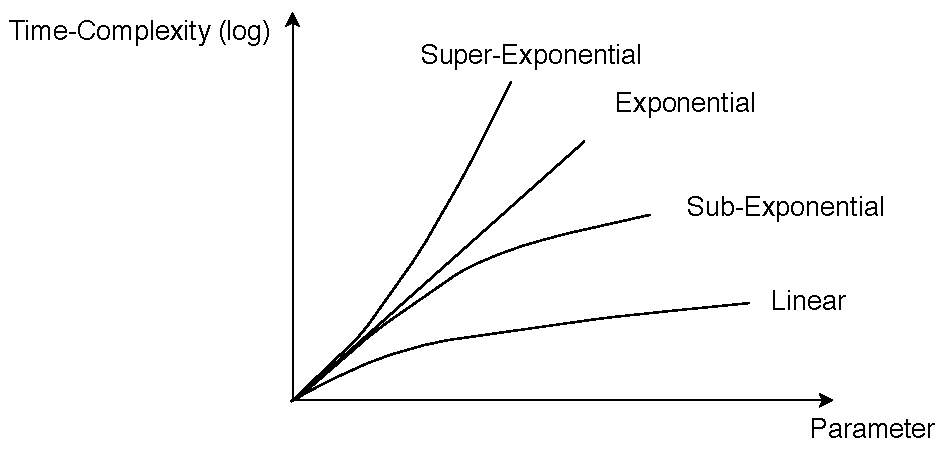
\includegraphics[width=0.8\textwidth]{files/Algorithm-Space.pdf}
%   \end{figure}
% }

\frame
{
  \frametitle{Introduction}

  The best SIS solver is exponential

  \begin{figure}[ht!]
  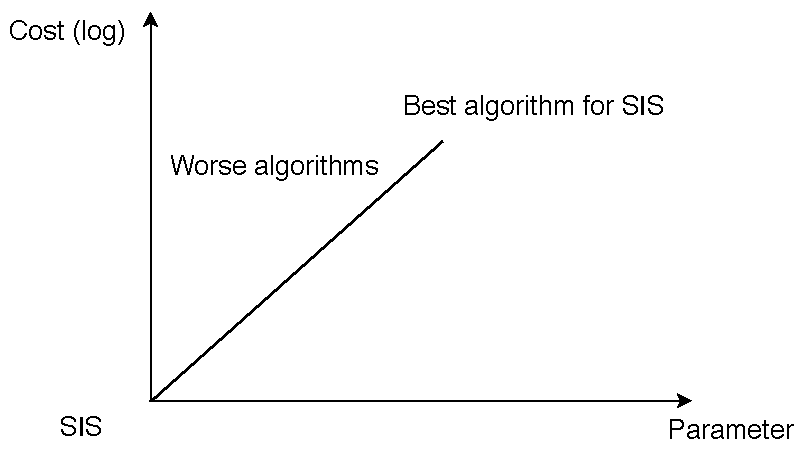
\includegraphics[width=0.8\textwidth]{files/SIS-Solvers.pdf}
  \end{figure}
}

\frame
{
  \frametitle{Introduction}

  \begin{itemize}
  	\item Reduction from SIS to Dilithium: Dilithium solver to SIS solver.
  	\item Attack Dilithium by SIS solver: SIS solver to Dilithium solver.
  \end{itemize}

  \begin{figure}[ht!]
  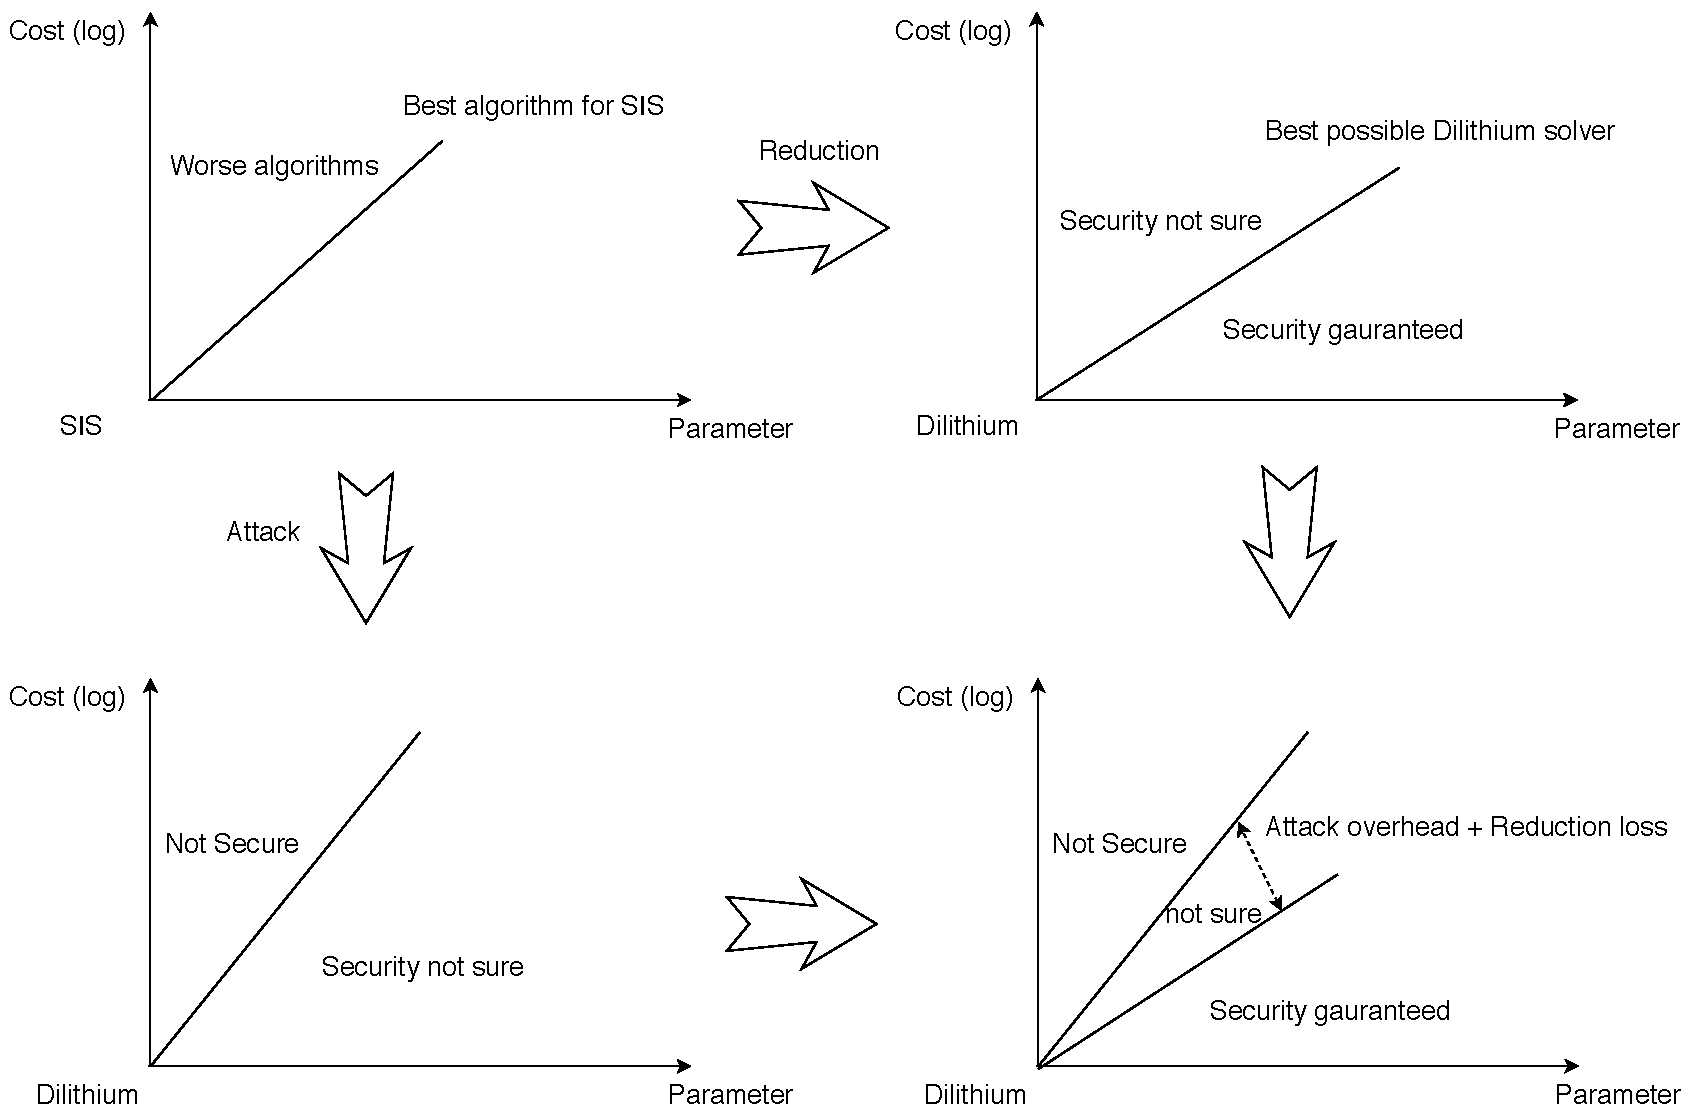
\includegraphics[width=0.8\textwidth]{files/SIS-Dilithium.pdf}
  \end{figure}
}

% \frame
% {
%   \frametitle{Concrete Security}
%   If technique improves, the graph will change in the following ways
%   \begin{itemize}
%   	\item Better attack to SIS using Dilithium $\Rightarrow$ guaranteed area increases
%   	\item Better attack to Dilithium using SIS $\Rightarrow$ insecure area increases
%   	\item Better attack to SIS $\Rightarrow$ security down in the whole
%   \end{itemize}
%   \begin{figure}[ht!]
%   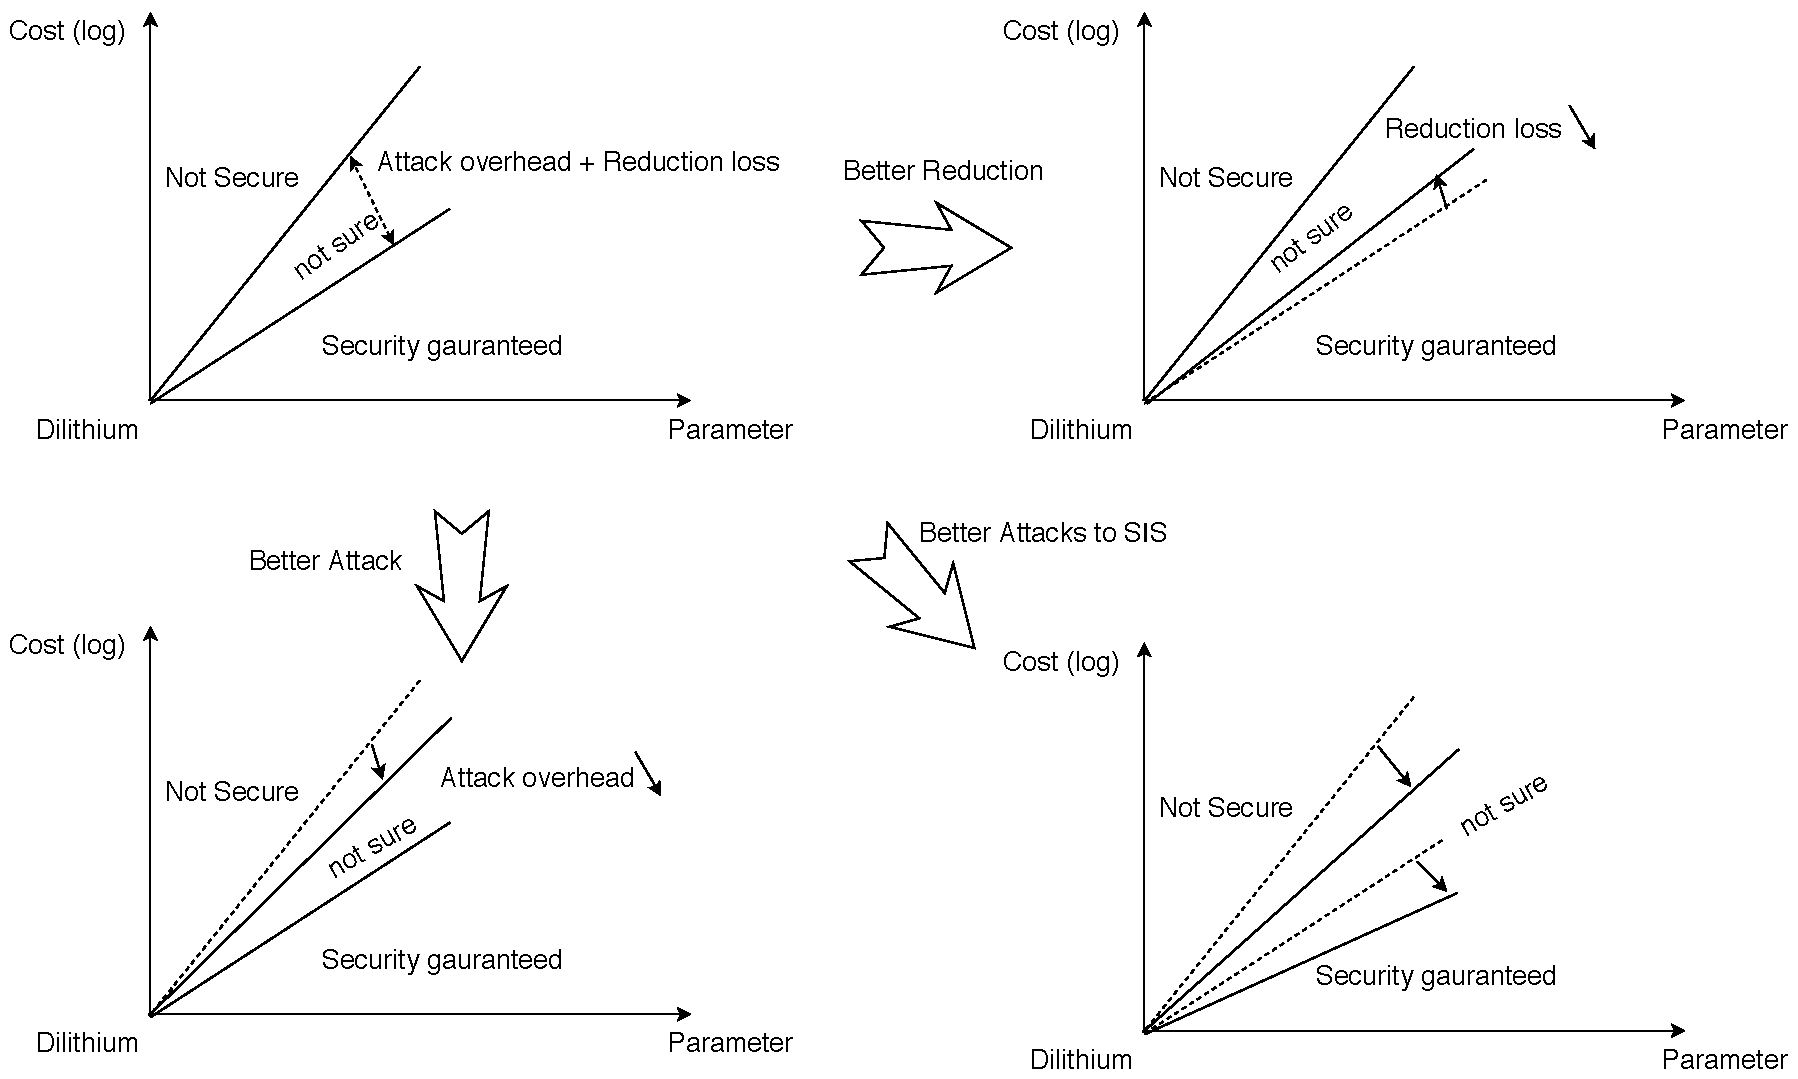
\includegraphics[width=0.8\textwidth]{files/Improved-Technique.pdf}
%   \end{figure}
% }

\frame
{
  \frametitle{Introduction}
  Determine the parameters for target security bits
  \begin{figure}[ht!]
  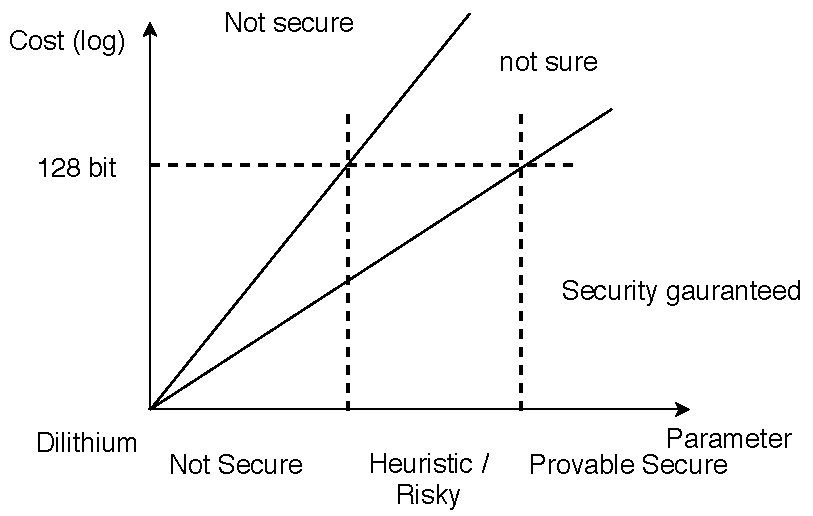
\includegraphics[width=0.5\textwidth]{files/Security-Bits.pdf}
  \end{figure}

  \begin{remark}
    Starting from this, we can
    \begin{enumerate}
    	\item Find better attacks, move the upper line to right, and prove the tightness of reduction
    	\item If better attacks are hard to find, we may try to find better reduction, and move the lower line to left
    \end{enumerate}
  \end{remark}
}

\section{Attack MSIS with BKZ}

\frame
{
  \frametitle{Attack MSIS with BKZ}
  Brief review of SIS
  \begin{figure}[ht!]
  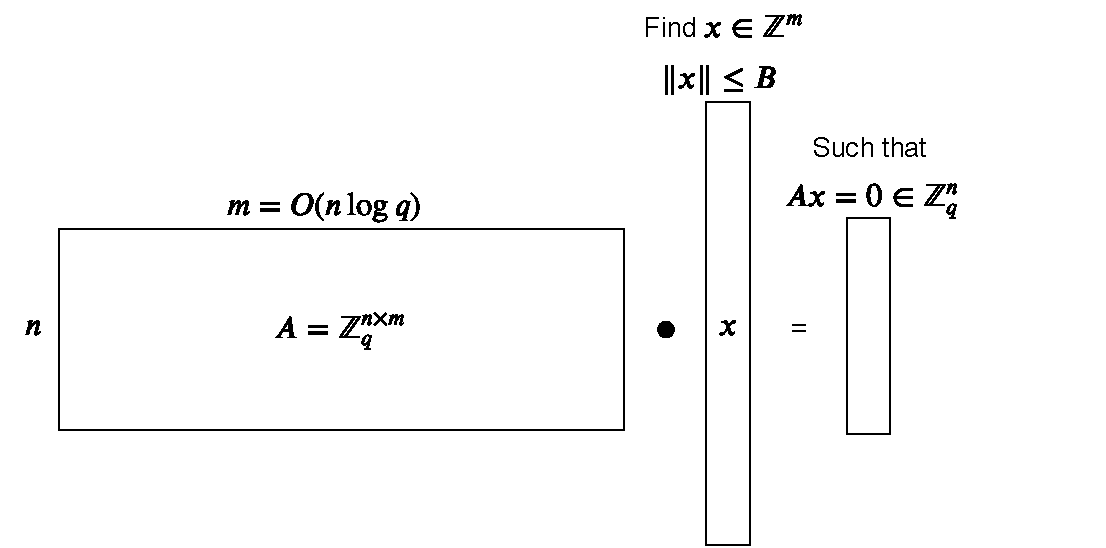
\includegraphics[width=0.8\textwidth]{files/SIS.pdf}
  \end{figure}

}

\frame
{
  \frametitle{Attack MSIS with BKZ}

  MSIS is generalization of SIS by replacing $\bbZ_q$ with ring $R_q$.
  \begin{itemize}
  	\item Currently no attack exploits the algebraic structure.
  	\item MSIS with parameters $m,n,q,d,B$ is considered as secure as SIS with parameters $m\cdot d,n\cdot d,q,B$
  \end{itemize}
  \begin{figure}[ht!]
  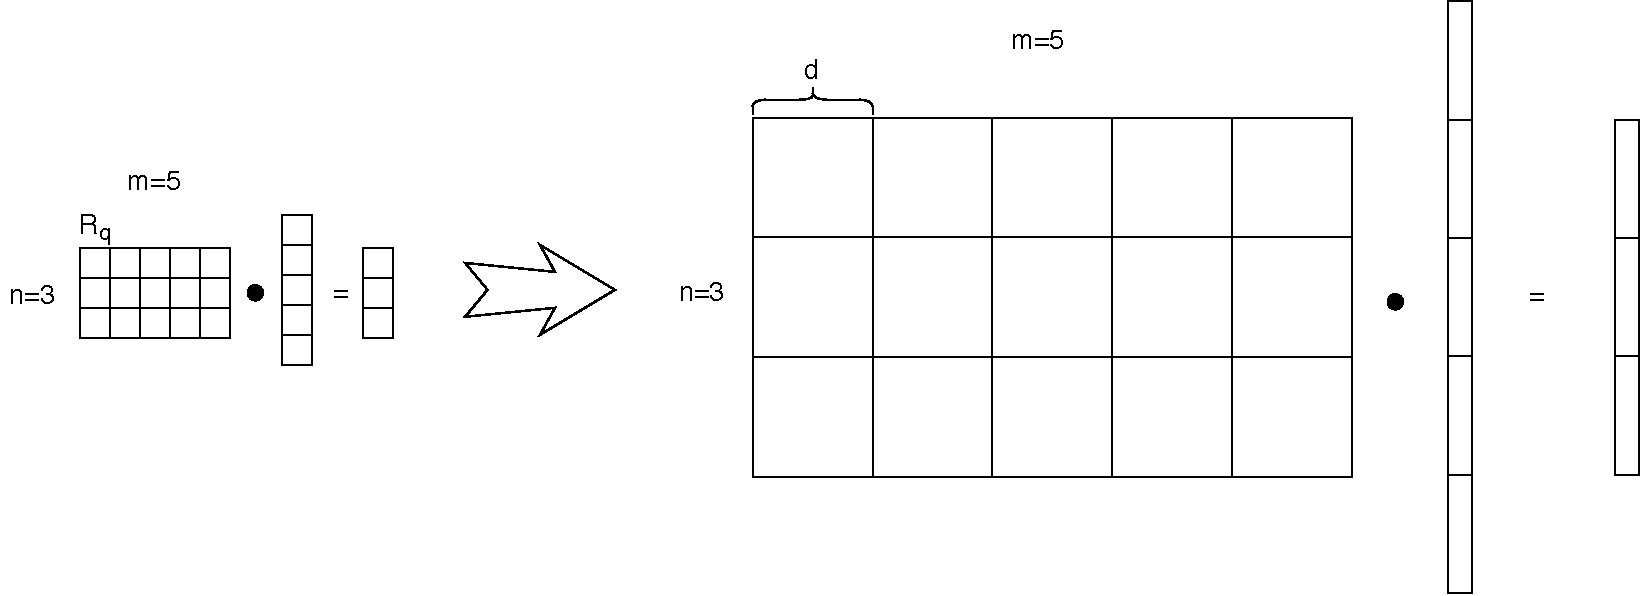
\includegraphics[width=\textwidth]{files/MSIS-SIS.pdf}
  \end{figure}
}

\frame
{
  \frametitle{Attack MSIS with BKZ}
  Euclidean-norm ($\ell_2$-SIS) v.s. Maximal-norm ($\ell_{\infty}$-SIS)
  \begin{itemize}
  	\item Since $(q,0,\cdots,0)$ is a solution, $B<q$ is required in both cases
  	\item For both of them, the best attack is to view the problem as SVP and solve it with BKZ
  	\item $\ell_2$-norm is always greater than $\ell_{\infty}$-norm, by scale of $\sqrt{m}$
  	\item For same security level, $B$ for $\ell_{\infty}$-SIS should be smaller than for $\ell_2$-SIS
  	\item BKZ focuses on the Euclidean norm, the security analysis of $\ell_{\infty}$-SIS under BKZ attack has not been studied in detail
  \end{itemize}

  \begin{remark}
  Dilithium relies on the $\ell_{\infty}$-MSIS
  \end{remark}
}

\frame
{
  \frametitle{Attack MSIS with BKZ}
  SIS as SVP
  \begin{itemize}
  	\item For $A\in\bbZ_q^{n\times m}$, the SIS problem is equivalent to finding a ``short'' vector in lattice
  		\[\cLp(A)=\{x\in\bbZ^m | Ax=0\bmod q\}\]
  	\item $\cLp(A)$ is a $q$-ary lattice, i.e. contains the lattice $q\mathbb{Z}^m$
  \end{itemize}

  Optimization
  \begin{itemize}
  	\item We do not have to use all $m$ columns. We can randomly select $w$ columns from it. For other columns, set the corresponding $x_i$ to $0$
  	\item Let $A_w$ denote the matrix formed by the selected $w$ columns, i.e. $A_w\in\bbZ_q^{n\times w}$
  \end{itemize}
}

\frame
{
  \frametitle{Attack MSIS with BKZ}
  Generate original set of vectors $\{\vb_i\in\cLp(A_w)\}_i^{N}$:
  \begin{itemize}
  	\item For $1\leq i\leq w$, let $\vb_i=q\vec{e}_i=(0,\cdots,0,q,0,\cdots,0)$
  	\item For $w<i\leq N$, generate solutions to $A_w\vec{x}=\vec{0}\bmod q$ uniformly randomly
  	\begin{itemize}
  		\item Uniformly randomly select first $w-n$ coordinates in $\bbZ_q$
  		\item Solve for the rest $n$ coordinates by linear algebra
  	\end{itemize}
  \end{itemize}

  The lengths $\{\ell_i\}$ after Gram-Schmidt orthogonalization has the following shape
  \begin{figure}[ht!]
  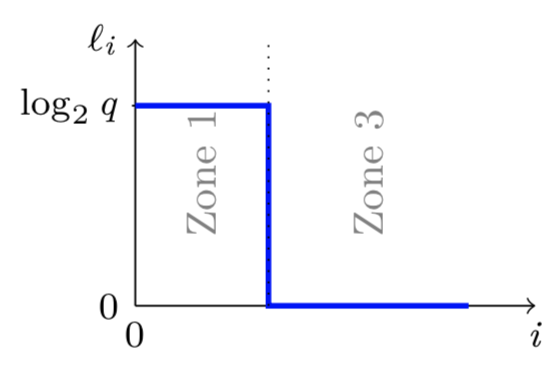
\includegraphics[width=0.4\textwidth]{files/before-reduction.png}
  \end{figure}
}

\frame
{
  \frametitle{Attack MSIS with BKZ}
  The BKZ rounds smoothify the GS length shape

  \begin{figure}[ht!]
  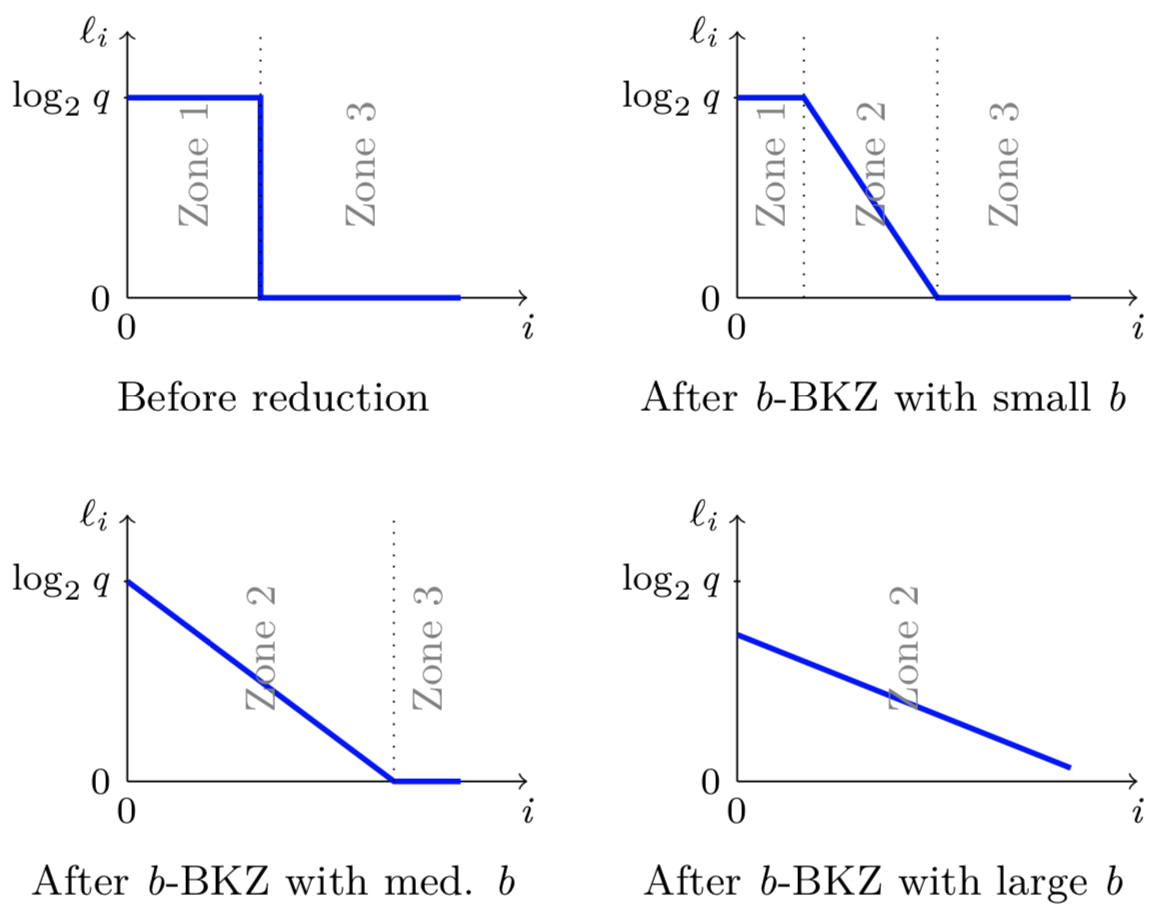
\includegraphics[width=0.7\textwidth]{files/bkz-sis.png}
  \end{figure}
}

\frame
{
  \frametitle{Attack MSIS with BKZ}
  The cost of BKZ in solving SIS is
  \[t_{BKZ}/\epsilon_{BKZ}\]
  \begin{itemize}
    \item $t_{BKZ}$ is the time of BKZ
    \item $\epsilon_{BKZ}$ is the probability that after BKZ reduction, at least one basis vector is bounded by $B$
  \end{itemize}
}

\frame
{
  \frametitle{Attack MSIS with BKZ}
  For simplicity, the Dilithium team estimates $t_{BKZ}$ by a single call to SVP solver on local block of size $\beta$
  \begin{itemize}
    \item The best asymptotic complexity is achieved by sieving: $\sqrt{4/3}^{\beta}$
    \item The Dilithium team believes that this estimate is at least 10 bits lower than actual security
  \end{itemize}
}

\frame
{
  \frametitle{Attack MSIS with BKZ}
  To estimate the probability $\epsilon_{BKZ}$, examine the shape of the basis vectors after BKZ reduction:
  \begin{itemize}
    \item Only consider the vectors in Zone 2, as they are the only vectors modified by BKZ
    \item These vectors, after projected orthogonally to vectors in Zone 1:
    \begin{itemize}
      \item Have $\ell_2$ norm $\approx 2^{\ell_i}$, where $i$ is the start of Zone 2
      \item Have the first $i-1$ coordinates being $0$
    \end{itemize}
  \end{itemize}
  \begin{figure}[ht!]
  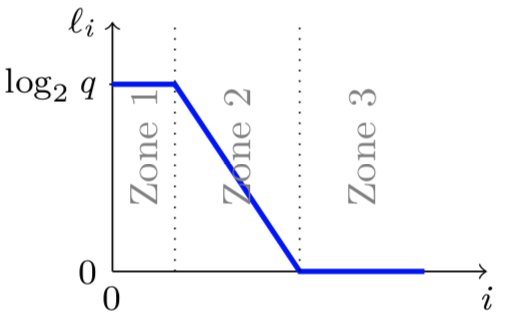
\includegraphics[width=0.4\textwidth]{files/after-reduction.png}
  \end{figure}
}

\frame
{
  \frametitle{Attack MSIS with BKZ}
  Statements claimed by Dilithium that are \alert{hard to understand}:
  \begin{itemize}
    \item We can obtain $\sqrt{4/3}^{\beta}$ vectors
    \item Let $j$ be the end of Zone 2, i.e. the maximal such that $\ell_j>0$, then the last $w-j$ coordinates (from $j+1$ to $w$) are $0$
  \end{itemize}
  From all above
  \begin{itemize}
    \item The middle $j-i+1$ coordinates have $\ell_2$ norm $\approx 2^{\ell_i}$
    \item Each coordinate is approximately of size $2^{\ell_i}/\sqrt{j-i+1}\approx q/\sqrt{j-i+1}$
  \end{itemize}
  Finally, each vector can be modeled as follows
  \begin{itemize}
    \item The first $i-1$ coordiantes modeled by uniform random distribution over $[-q/2, q/2]$
    \item The middle $j-i+1$ coordinates modeled by discrete normal distribution with $\sigma=q/\sqrt{j-i+1}$
  \end{itemize}
}

\frame
{
  \frametitle{Attack MSIS with BKZ}
  The probability that at least one vector is within bound $B$ is approximately
  \[
  	 \epsilon_{BKZ}:=1-\left(1-\left(\frac{2B+1}{q}\right)^{i-1}\left(2\Phi\left(\frac{B\sqrt{j-i+1}}{q}\right)-1\right)^{j-i+1}\right)^{\sqrt{4/3}^{\beta}}\,
  \]
  where $\Phi(\cdot)$ is the CDF of standard normal distribution.
}

\frame{
	\center
	\large{Q \& A}
}

\end{document}
